%&latex
\documentclass[notes=show]{beamer}
%%%%%%%%%%%%%%%%%%%%%%%%%%%%%%%%%%%%%%%%%%%%%%%%%%%%%%%%%%%%%%%%%%%%%%%%%%%%%%%%%%%%%%%%%%%%%%%%%%%%%%%%%%%%%%%%%%%%%%%%%%%%%%%%%%%%%%%%%%%%%%%%%%%%%%%%%%%%%%%%%%%%%%%%%%%%%%%%%%%%%%%%%%%%%%%%%%%%%%%%%%%%%%%%%%%%%%%%%%%%%%%%%%%%%%%%%%%%%%%%%%%%%%%%%%%%
\usepackage{amssymb}
\usepackage{mathpazo}
\usepackage{hyperref}
\usepackage{multimedia}
\usepackage{graphicx}
\usepackage{amssymb}
%\usecolortheme[named=black]{structure}
%\usetheme[height=10mm]{Rochester}
\usetheme{CambridgeUS}
%\input{tcilatex}
\begin{document}

\title[]{ECB's Target claims and liabilities: A cause or a reflection of the current Euro crisis?}
\author[]{J\o rn Inge Halvorsen \inst{1}}
\institute[]{Norwegian Business School (BI)}
\date[]{28. September, 2012}
\maketitle
\section{Present situation}
\begin{frame}
\frametitle{Economics of Monetary Union}
\begin{itemize}
\item The policy debate about the Euro crisis seems to be founded mainly on results  discusses in standard textbooks on the economics of monetary union (see for e.g. \cite{de2012economics}   aul De Grauwe).\begin{itemize}
\item Partial equilibrium analysis.
\item Discussion usually within a IS-LM model framework.
\item Rely on different shortcuts
\end{itemize}
\item Hans Werner Sinn and Timo Wolmershauser (2012) argue that the failure of the Euro lies more in the initial set-up of the whole system.
\begin{itemize}
\item Democratic voting system within the Eurozone (one country one vote)\\
\item Unconventional monetary policy tools
\item \textbf{Market vs. monetary interventions }
\item Legal issues
\item Redistribution between agents
\end{itemize}\end{itemize}
\end{frame}
\cite{smets2010shocks}
\frametitle{For further reading:}
\begin{thebibliography}{10}
\bibitem[Smets, F. and Wouters, R., 2010]{smets2010shocks}
Smets, F. and Wouters, R.
\newblock Shocks and frictions in US business cycles: A Bayesian DSGE approach
\end{thebibliography}
\end{document}

\end{document}

\frametitle{For further reading:}
\begin{thebibliography}{10}
@book{de2012economics,
  title={Economics of monetary union},
  author={De Grauwe, P.},
  year={2012},
  publisher={OUP Oxford}
}
\end{thebibliography}
Test
\end{document}

\begin{frame}
\frametitle{Sovereign debt and interest rate spreads}
\includegraphics[width=\textwidth]{debtgdp.png}
\end{frame}
\bibliographystyle{econometrica}%
\bibliography{target}%

\begin{frame}
\frametitle{Sovereign debt and interest rate spreads}
\includegraphics[width=\textwidth]{spread.png}
\end{frame}
\begin{frame}
\frametitle{Sovereign debt and interest rate spreads}
\begin{itemize}
\item Is the Euro crisis purely a sovereign debt crisis?
\begin{itemize}
\item Only before the fianciansd
\end{itemize}
\item The P(I)IGS also suffer from external imbalances
\begin{itemize}
\item Credit expansion
\item Credit stopped
\item Today: Need for a price realignment.
\end{itemize}
\end{itemize}
\end{frame}
\section{Target claims and liabilities}
\begin{frame}
\frametitle{The Balance of Payments}
\begin{itemize}
\item The BOP equation under different monetary policy regimes:
\begin{itemize}
\item Floating
\begin{equation*}
0 \equiv \text{CUR.ACC.} + \text{CAP.ACC.}
\end{equation*}
\item Fixed
\begin{equation*}
\Delta\text{RES.} \equiv \text{CUR.ACC.} + \text{CAP.ACC.}
\end{equation*}
\item Eurozone
\begin{equation*}
\Delta\text{TC} \equiv \text{CUR.ACC.} + \text{CAP.ACC.}
\end{equation*}
\end{itemize}
\end{itemize}
Target claims and liabilities (TC) representing accumulated intra-Eurozone balance of payments.
\end{frame}
\begin{frame}
\frametitle{}
\includegraphics{targetcl.png}
\begin{itemize}
\item  Target claims are (low ) interest rate bearing assets without any formal redemption possibilities (unlike the federal reserve system).
\item System theoretically sustainable, but politically?
\item Sinn Wolmershauser: (2012): The Eurocrisis is a balance of payment crisis.
\end{itemize}
\end{frame}
\section{Bretton Woods as a parallel}
\begin{frame}
\frametitle{}
\begin{itemize}
\item Bretton Woods: Monetary agreement between the US and its allies after the Second World war
\item Initial set-up of the system
\begin{itemize}
\item US dollar redeemable towards gold
\item Other countries currency fixed towards dollar
\item No direct regulations on money supply growth
\end{itemize}
\end{itemize}
\end{frame}
\begin{frame}
%\frametitle{ The process of outside money creation}
\includegraphics[width=\textwidth]{balsheetbw.eps}
\end{frame}
\begin{frame}
\frametitle{}
\begin{itemize}
\item Imbalances in the system started from 1958
\item De Gaule: Redeem US reserves for gold.
\item 1971 US dollar no longer redeamble towards the dollar.
\item End of Bretton Woods
\end{itemize}
\end{frame}
\section{Differences}
\begin{frame}
\frametitle{Main differences between Bretton Woods and the EBS system}
\begin{itemize}
\item The �conversation ratio� is 1:1 between the currencies
\item Transactions today mainly electronical (Target 2-system)
\item Target claims are without formal redemption possibilities
\item ECB council total control over money base creation
\end{itemize}
\end{frame}
\begin{frame}
\frametitle{}
\includegraphics[width=\textwidth]{balsheetez}
\end{frame}
\section{Market interventions and TC}
\begin{itemize}
\item Note: Without money base creation the Target claims would be zero for all
\item Target credit represent a combination of conventional and unconventional monetary policy
\item As, put the "exogenous" variable on the righ hand side we can write
\begin{equation*}
\text{CUR.ACC.} + \text{CAP.ACC.}\equiv \Delta\text{TC}
\end{equation*}
\item Monetary policy invention: Two extreme cases
\begin{enumerate}
\item Electronic Money growth with capital market shut down
\begin{equation*}
\text{CUR.ACC.} \equiv \Delta\text{TC}
\end{equation*}
$\Rightarrow $ Fiances current account deficit
\item Higher interest rate since must be finances by privat capital
\begin{equation*}
\text{CAP.ACC.} \equiv \Delta\text{TC}
\end{equation*}
Higher interest rate since must be finances by privat capital
\end{enumerate}
\end{itemize}
\section{The case for the PIIGS economies?}
\begin{frame}
\frametitle{}
\includegraphics[width=\textwidth]{tc_ca_cu.png}
\end{frame}
\begin{frame}
\frametitle{}
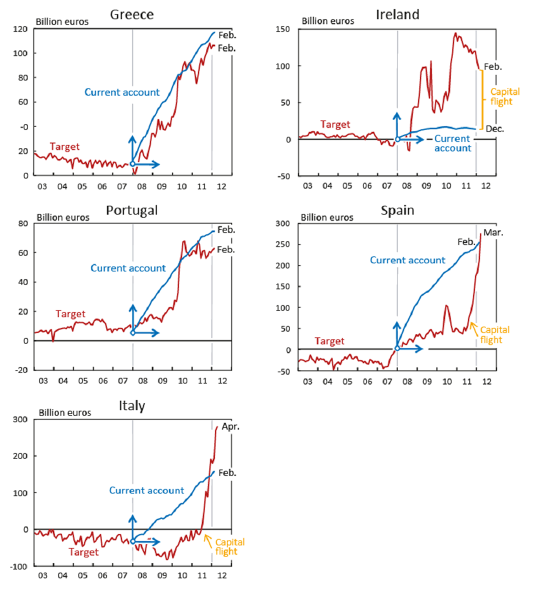
\includegraphics[width=\textwidth]{TC_CA_CU_PIIGS}
\end{frame}
\begin{frame}
\frametitle{The way ahead?}
\begin{itemize}
\item Policy of relaxed budget constraints
\begin{itemize}
\item Let the present system continue
\item Common bonds
\end{itemize}
\item Return to markets
\begin{itemize}
\item Gradually make target claims redeemable towards marketable assets
\item Exit of the eurozone
\end{itemize}
\end{itemize}
\end{frame}
\end{document}



